\begin{frame}
	\frametitle{Motivación}
	
	Don’t reinvent the wheel. Create something new and do it faster and better by building on ROS!
	
	\note{https://www.ros.org/blog/why-ros/}
	
	\note{http://wiki.ros.org/es/ROS/Tutoriales}
	
	\note{https://www.youtube.com/playlist?list=PL8dDSKArO2-m7hAjOgqL5uV75aZW6cqE5}
	
\end{frame}

\begin{frame}
	\frametitle{¿Qué es ROS?}
	
	ROS (Robot Operating System) es un kit de desarrollo de software de código abierto para aplicaciones de robótica. ROS ofrece una plataforma de software estándar para desarrolladores de todas las industrias que los llevará desde la investigación y la creación de prototipos hasta la implementación y la producción.
	
	\begin{itemize}
		\item Comunidad global
		\item Utilizado en cursos de robótica, investigación e industria
		\item Acorta los tiempos de producción
		\item Multi-dominio: indoor / outdoor, hogareño / industrial, bajo el agua / espacio
		\item Multi-plataforma: Linux, Windows y macOS.
		\item Open-source
		\item Licencia permisiva (Apache 2.0)
		\item Soporte desde la industria
	\end{itemize}
	
	
	\note{https://www.ros.org/blog/why-ros/}
	
	
\end{frame}

\begin{frame}
	\frametitle{¿Qué es ROS?}
	  Trabajaremos con la versión Ubuntu LTS más actual, esta siempre viene con una versión de ROS estable.
	
	\begin{figure}[!h]
		\centering
		\subfloat[ROS1]
		{
			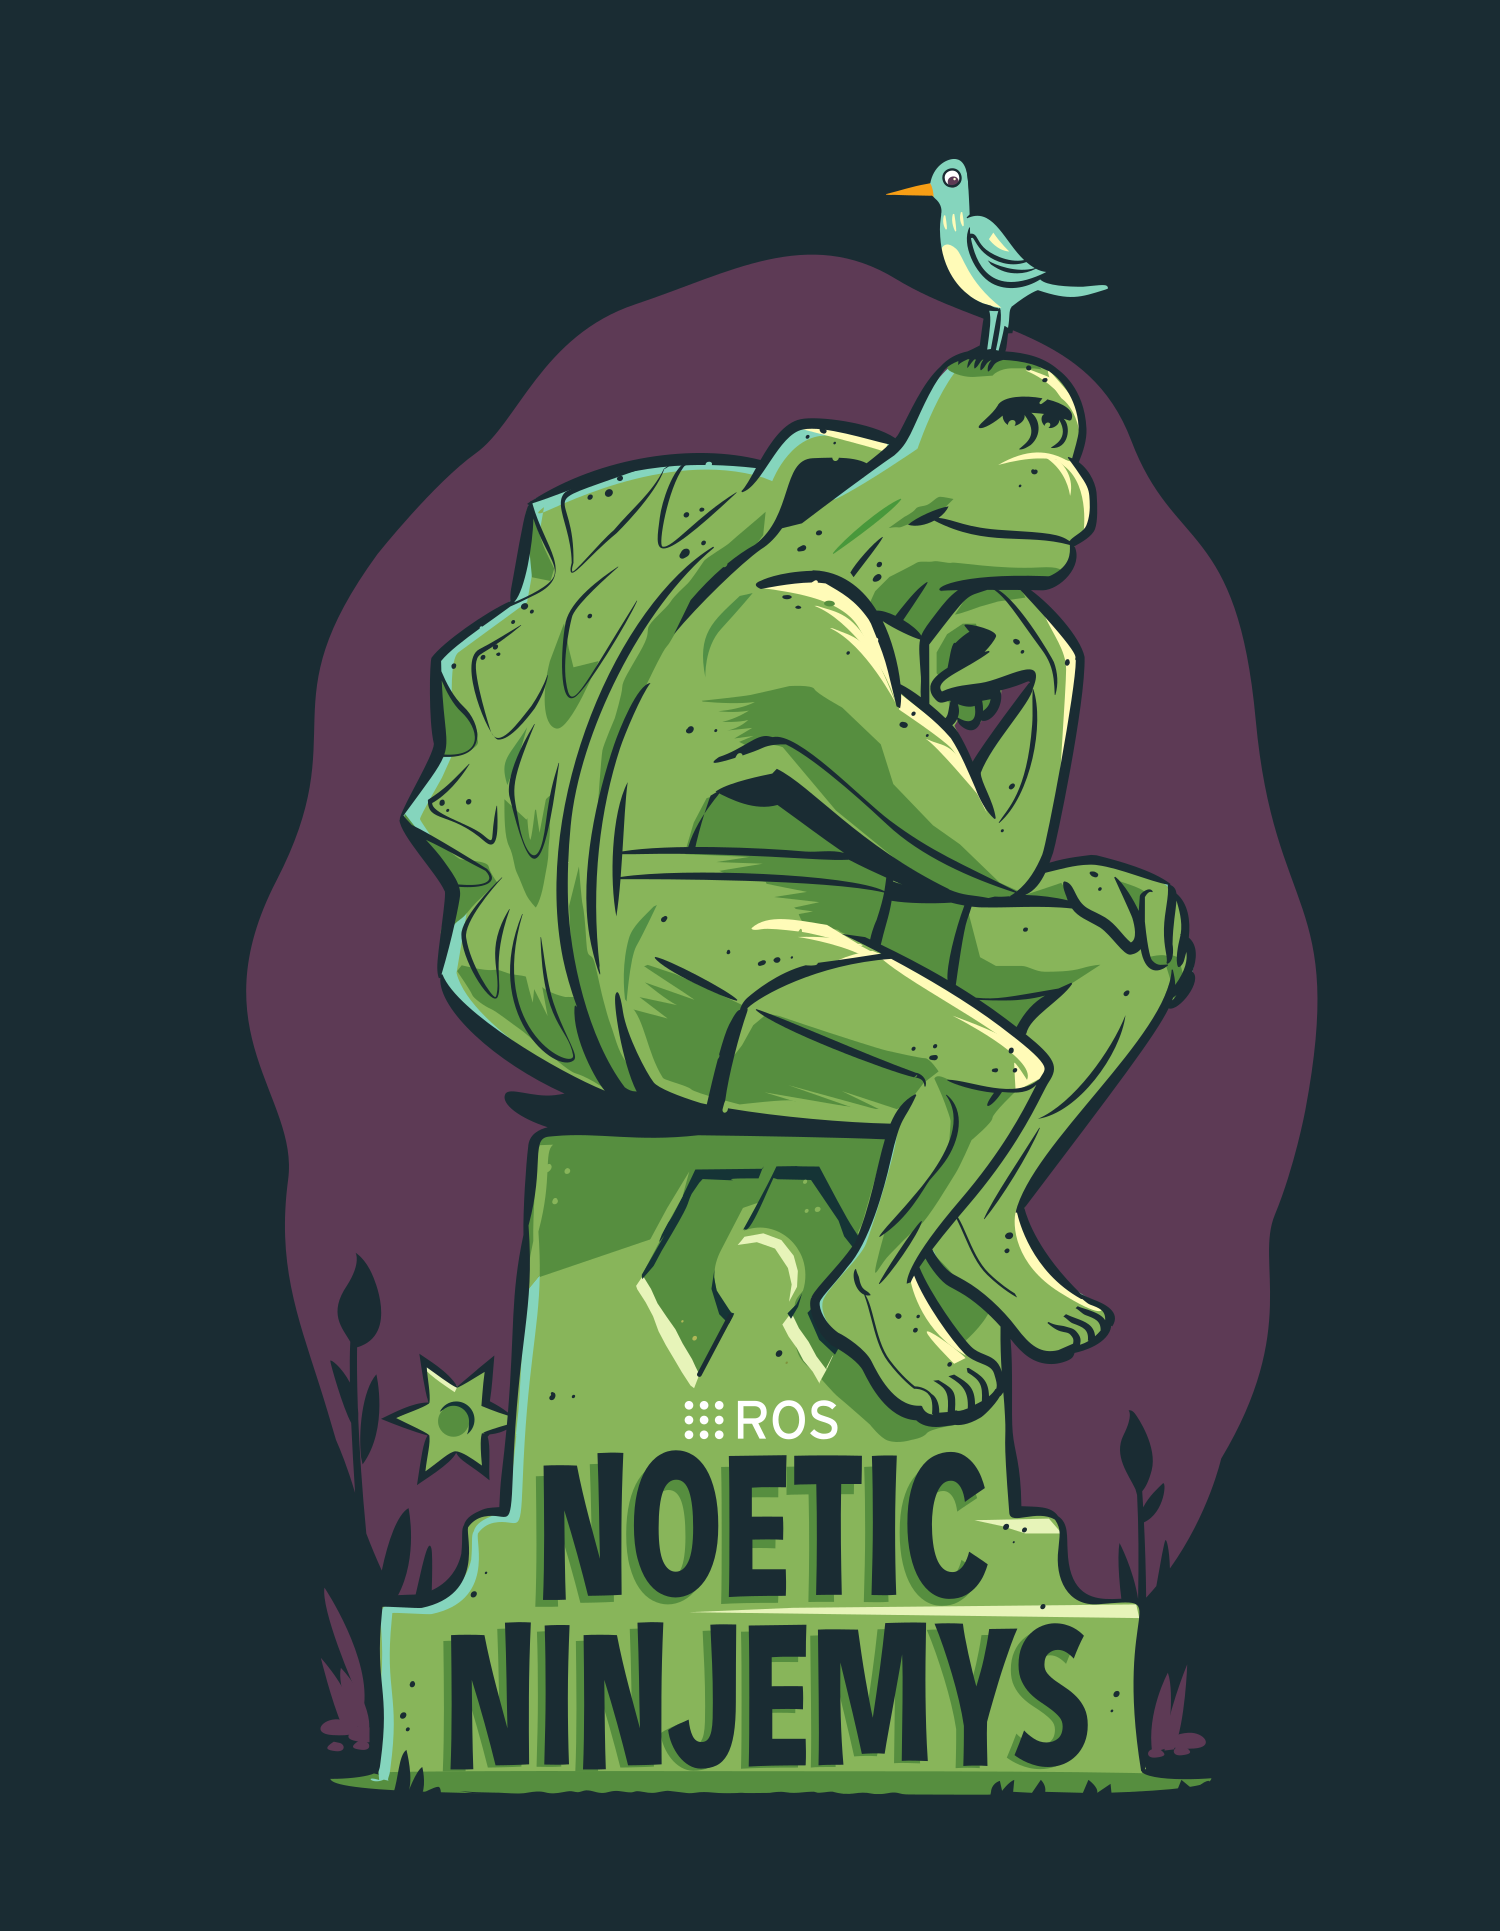
\includegraphics[width=0.4\columnwidth]{images/ros_version_noetic.png}
		}
		\subfloat[ROS2]
		{
			
\includegraphics[width=0.4\columnwidth]{images/ros_version_humble.png}
		}
	\end{figure}

\end{frame}

\begin{frame}
	\frametitle{Configuración de entorno de ROS}
    
    https://docs.ros.org/en/<distro>/Tutorials.html
    
    Instalar ROS
    
    sudo apt install ros-<distro>-<package>
    
    Sourcear los archivos de setup
    
    source /opt/ros/<distro>/setup.bash
    
    Agregar el source al .bashrc
    
    echo "source /opt/ros/<distro>/setup.bash" >> ~/.bashrc
    
    Chequear las variables de entorno
    
    printenv | grep -i ROS
    
    Output:
    
    ROS\_VERSION=2\\
    ROS\_PYTHON\_VERSION=3\\
    ROS\_DISTRO=humble
    
    

    setear el DOMAIN ID:
    
    Los nodos ROS 2 en el mismo dominio pueden descubrir y enviarse mensajes libremente, mientras que los nodos ROS 2 en diferentes dominios no pueden. Todos los nodos ROS 2 utilizan el ID de dominio 0 de forma predeterminada.
    
    echo "export ROS\_DOMAIN\_ID=<your\_domain\_id>" >> ~/.bashrc
	
	
\end{frame}

\begin{frame}
	\frametitle{Creando un paquete en ROS}
	
     Building system: ament
     luego para compilar un paquete: colcon build
     
     
     crear un paquete:
     
     ros2 pkg create test\_pkg --build-type ament\_cmake
	
\end{frame}

\begin{frame}
	\frametitle{Cómo escribir un Publicador y un subscriptor}

\end{frame}


\begin{frame}
	\frametitle{Install turtlebot en ROS}
	
\end{frame}

\begin{frame}
	\frametitle{Publicar velocidades a Turtlebot}
	
\end{frame}

\begin{frame}
	\frametitle{TF}
	Hablar de las TF de ROS.
	
\end{frame}

\begin{frame}
	\frametitle{Rosbags}
	topic node hz echo Bw etc...
	
\end{frame}

\begin{frame}
	\frametitle{RViz}
	topic node hz echo Bw etc...
	
\end{frame}

\begin{frame}
	\frametitle{Crear mensajes customizados}
	Hablar de las TF de ROS.
	
\end{frame}

\begin{frame}
	\frametitle{Herramientas por línea de comandos útiles}
    topic node hz echo Bw etc...
    ros2 <hit\_tab>
    ros2 topic list
    ros2 bag 
	
\end{frame}
